\documentclass[dvipdfmx]{jsarticle}


\usepackage{tcolorbox}
\usepackage{color}
\usepackage{listings, plistings}

%% ノート/latexメモ
%% http://pepper.is.sci.toho-u.ac.jp/pepper/index.php?%A5%CE%A1%BC%A5%C8%2Flatex%A5%E1%A5%E2

%% JavaScriptの設定
%% https://e8l.hatenablog.com/entry/2015/11/29/232800
\lstdefinelanguage{javascript}{
  morekeywords = [1]{ %keywords
    await, break, case, catch, class, const, continue, debugger, default, delete, 
    do, else, enum, export, extends, finally, for, function, function*, if, implements, import, in, 
    instanceof, interface, let, new, package, private, protected, public, return, static, super,
    switch, this, throw, try, typeof, var, void, while, with, yield, yield*
  },
  morekeywords = [2]{ %literal
    false, Infinity, NaN, null, true, undefined
  },
  morekeywords = [3] { %Classes
    Array, ArrayBuffer, Boolean, DataView, Date, Error, EvalError, Float32Array, Float64Array,
    Function, Generator, GeneratorFunction, Int16Array, Int32Array, Int8Array, InternalError,
    JSON, Map, Math, Number, Object, Promise, Proxy, RangeError, ReferenceError, Reflect,
    RegExp, Set, String, Symbol, SyntaxError, TypeError, URIError, Uint16Array, Uint32Array,
    Uint8Array, Uint8ClampedArray, WeakMap, WeakSet
  },
  morecomment = [l]{//},
  morecomment = [s]{/*}{*/},
  morestring = [b]{"},
  morestring = [b]{'},
  alsodigit = {-},
  sensitive = true
}

%% 修正時刻: Tue 2022/03/15 10:04:41


% Java
\lstset{% 
  frame=single,
  backgroundcolor={\color[gray]{.9}},
  stringstyle={\ttfamily \color[rgb]{0,0,1}},
  commentstyle={\itshape \color[cmyk]{1,0,1,0}},
  identifierstyle={\ttfamily}, 
  keywordstyle={\ttfamily \color[cmyk]{0,1,0,0}},
  basicstyle={\ttfamily},
  breaklines=true,
  xleftmargin=0zw,
  xrightmargin=0zw,
  framerule=.2pt,
  columns=[l]{fullflexible},
  numbers=left,
  stepnumber=1,
  numberstyle={\scriptsize},
  numbersep=1em,
  language={Java},
  lineskip=-0.5zw,
  morecomment={[s][{\color[cmyk]{1,0,0,0}}]{/**}{*/}},
  keepspaces=true,         % 空白の連続をそのままで
  showstringspaces=false,  % 空白字をOFF
}
%\usepackage[dvipdfmx]{graphicx}
\usepackage{url}
\usepackage[dvipdfmx]{hyperref}
\usepackage{amsmath, amssymb}
\usepackage{itembkbx}
\usepackage{eclbkbox}	% required for `\breakbox' (yatex added)
\usepackage{enumerate}
\usepackage[default]{cantarell}
\usepackage[T1]{fontenc}
\fboxrule=0.5pt
\parindent=1em
\definecolor{mygrey}{rgb}{0.97, 0.97, 0.97}

\makeatletter
\def\verbatim@font{\normalfont
\let\do\do@noligs
\verbatim@nolig@list}
\makeatother

\begin{document}

%\anaumeと入力すると穴埋め解答欄が作れるようにしてる。\anaumesmallで小さめの穴埋めになる。
\newcounter{mycounter} % カウンターを作る
\setcounter{mycounter}{0} % カウンターを初期化
\newcommand{\anaume}[1][]{\refstepcounter{mycounter}{#1}{\boxed{\phantom{aa}\textnormal{\themycounter}\phantom{aa}}}} %穴埋め問題の空欄作ってる。
\newcommand{\anaumesmall}[1][]{\refstepcounter{mycounter}{#1}{\boxed{\tiny{\phantom{a}\themycounter \phantom{a}}}}}%小さい版作ってる。色々改造できる。

%% 修正時刻: Tue 2022/03/15 10:04:411


\section{IISの動作を止める}

XAMPPのコントロールパネルでApacheを起動しようと Start ボタンをクリック
しても、Apacheが起動しないことがある。

\vspace{3mm}
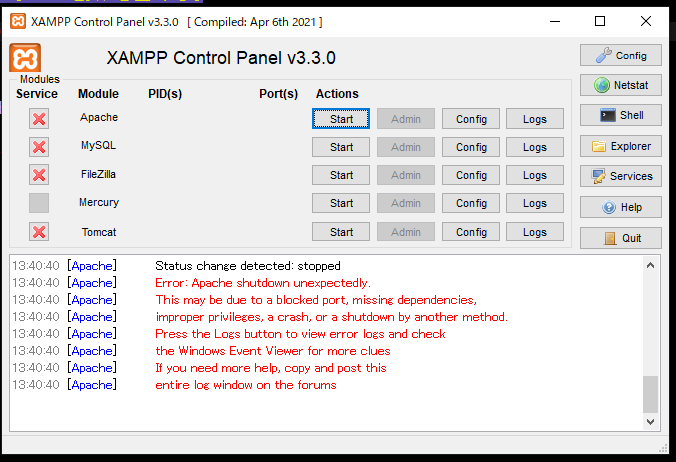
\includegraphics[width=10cm]{img/apache-error.png}
\vspace{3mm}

これは、Apacheが使用する80番と443番ポートが、すでに他のアプリによって
使用されているためかもしれない。

Windowsのタスクバーの検索で、``Windowsの機能の有効化または無効化''を
検索する。

すると、以下のようなダイアログが表示されるので、
``インターネット・インフォーメーション・サービス''の項目を見てみる。

黒くなっていたら、その''+''をクリックして展開し、
``World Wide Webサービス''の黒をクリックして白くする。
そして、OKとする。

\vspace{3mm}
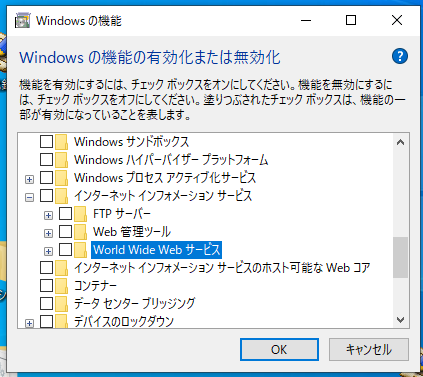
\includegraphics[width=10cm]{img/win-iis.png}
\vspace{3mm}

すると、インターネット・インフォーメーション・サービスを停止できるので、
80番ポート、443番ポートが開放されるので、Apacheが起動できる。


\section{MySQLをサービスに登録する}

MariaDB(MySQL)を停止させずに Windowsを終了させると、MariaDBのテーブルが
壊れやすくなると言われている。また、身近にもそういうケースが見られる。

そこで、mysqlをWindowsのサービスに登録する。
サービスに登録すれば、Windowsは終了時にサービスに登録しているプロセスを
停止させるだろうからである。

MySQLをサービスに登録するには、\textbf{C:\yen xampp\yen mysql} にある
``mysql\_installservice.bat''を使う。これは、mysqlをサービスに登録する
ためのスクリプトである。

ただ、このファイルの中を修正しなければならない点が1つある。
このファイルをTerapadなどのエディタで開く。

\begin{lstlisting}[title=mysql\_installservice.bat, language=bash]
 ... (略) ...
 
28 :MainNT
29 echo Installing MySQL as an Service 
30 copy "%cd%\bin\my.cnf" /-y %windir%\my.ini
31 bin\mysqld --install mysql --defaults-file="%cd%\bin\my.ini"
32 echo Try to start the MySQL deamon as service ... 
33 net start MySQL

 ... (略) ...
\end{lstlisting}

これの31行目の ``\verb!bin\mysqld!'' を
``\verb!bin\mysqld.exe!'' に変更する。

それから、コマンドプロンプトを 管理者権限で起動し、``C:\yen xampp\yen mysql''
に移動する。

\begin{lstlisting}
 C:\Widows\System32> cd C:\xampp\mysql
 C:\xampp\mysql>
\end{lstlisting}

そこで、``mysql\_installservice.bat''を実行する。

\begin{lstlisting}
 C:\xampp\mysql> mysql_installservice.bat
\end{lstlisting}

これで、mysql をサービスに登録できた。

\vspace{3mm}
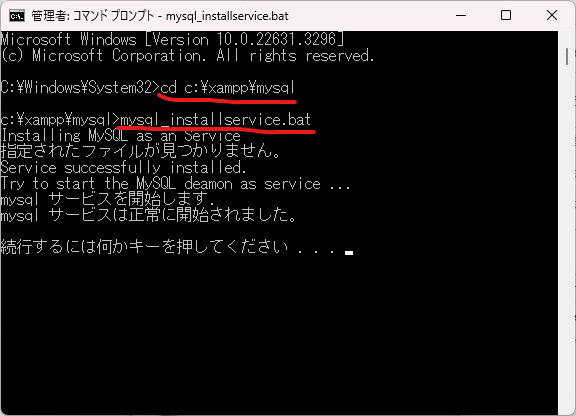
\includegraphics[width=10cm]{../02-install/23-mysql-installservice.png}
\vspace{3mm}


\begin{tcolorbox}[title=注意]
 mysql\_installservice.bat を右クリック--- 管理者権限で実行、では、
 うまくいかない。
\end{tcolorbox}

XAMPPコントロールパネルを起動しなおすと、mysqlが動作しているのがわかる。


\end{document}

%% 修正時刻: Sat May  2 15:10:04 2020


%% 修正時刻: Fri 2024/03/22 21:11:150
